
\section{CROW: Code Randomization of WebAssembly bytecode}
\label{section:crow}

% Overview
This section describes the red squared tooling in \autoref{diagrams:generic} named, CROW  \cite{CROW}. CROW is a tool tailored to create semantically equivalent \wasm variants from an LLVM front-end output.
Using a custom Wasm LLVM backend, it generates the Wasm binary variants.


In \autoref{diagrams:crow}, we describe the workflow of CROW to create program variants.
The Diversifier in CROW is composed by two main processes, \textit{exploration} and \textit{combining}. 
The \emph{exploration} process operates at the instruction level for each function in its input LLVM.
For each instruction, CROW produces a collection of functionally equivalent code replacements.   
In the \emph{combining} stage, CROW assembles the code replacements to generate different LLVM IR variants.
CROW generates the LLVM IR variants by traversing the power set of all possible combinations of code replacements.
Finally, the custom Wasm LLVM backend compiles the assembled LLVM IR variants into \wasm binaries.
In the following, we describe our design decisions. All our implementation choices are based on one premise: \emph{each design decision should increase the number of \wasm variants that CROW creates.}
%\subsection*{Overview}

\begin{figure*}[h]
    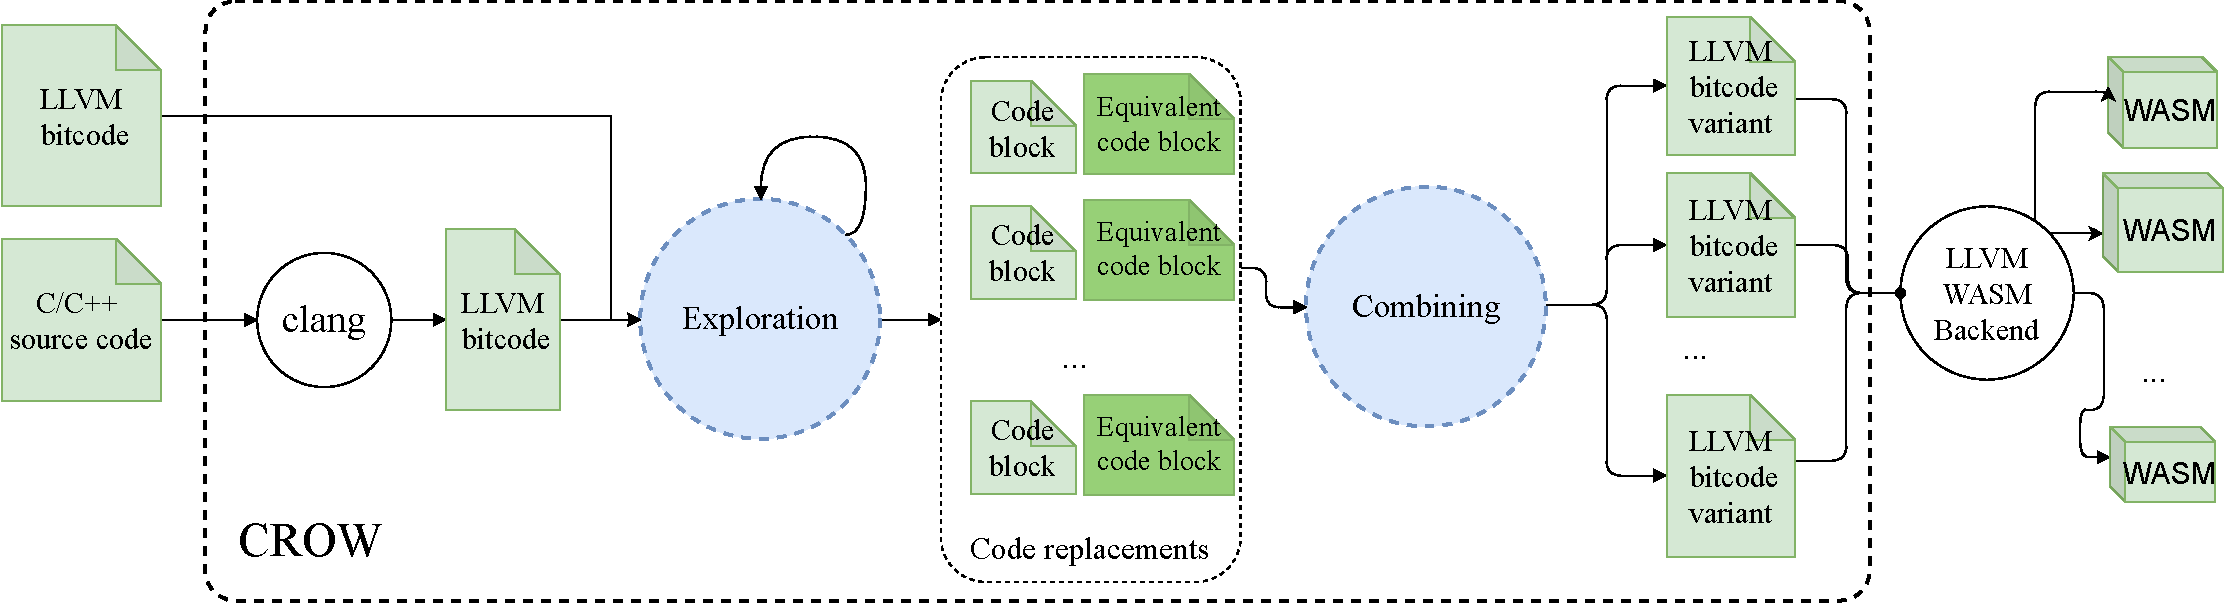
\includegraphics[width=\linewidth]{diagrams/generation/crow.drawio.pdf}
    \caption{CROW components following the diagram in \autoref{diagrams:generic}. CROW takes LLVM IR to generate functionally equivalent code replacements. Then, CROW assembles program variants by combining them.}
    \label{diagrams:crow}
\end{figure*}


%CROW operates at the code block level, taking them from the functions defined inside the input LLVM bitcode module. 
%In addition, the retargeted superoptimizer is in charge of finding the potential places in the original code blocks where a replacement can be applied. Finally, we use the enumerative synthesis strategy of the retargeted superoptimizer to generate code replacements.
%The code replacements generated through synthesis are verified, according to \autoref{def:functional-equivalence}, by internally using a theorem prover. 

\subsection{Exploration}

%\subsection*{Variants' generation}

The primary component of CROW's exploration process is its code replacements generation strategy. The diversifier implemented in CROW is based on the superdiversifier of Jacob \etal \cite{jacob2008superdiversifier}.
A superoptimizer focuses on \emph{searching} for a new program that is faster or smaller than the original code while preserving its functionality.
The concept of superoptimizing a program dates back to 1987, with the seminal work of Massalin \cite{Massalin1987} which proposes an exhaustive exploration of the solution space. The search space is defined by choosing a subset of the machine's instruction set and generating combinations of optimized programs, sorted by code size in ascending order. If any of these programs are found to perform the same function as the source program, the search halts. On the contrary, a superdiversifier keeps all intermediate search results despite their performance. 

% Why and main change
We use the superdiversifier idea of Jacob and colleagues to implement CROW because two main reasons.
First, the code replacements generated by this technique outperform diversification strategies based on hand-written rules. Besides, this technique is fully automatic.
Second, there is a battle-tested superoptimizer for LLVM, Souper \cite{Sasnauskas2017Souper:Superoptimizer}. This latter makes feasible the construction of a generic LLVM superdiversifier. 

% This paragraph is hard to read
% How Souper works and why we can modify if
% Souper works as follows.
We modify Souper to keep all possible solutions in their searching algorithm.
Souper builds a Data Flow Graph for each LLVM integer-returning instruction. 
Then, for each Data Flow Graph, Souper exhaustively builds all possible expressions from a subset of the LLVM IR language.
Each syntactically correct expression in the search space is semantically checked versus the original with a theorem solver. Souper synthesizes the replacements in increasing size. Thus, the first found equivalent transformation the optimal replacement result of the searching. 
We keep more equivalent replacements during the searching by removing the halting criteria. Instead, we limit the searching for a replacement with timeout and the replacement's size. Our customized Souper reports a new code replacement as soon as an equivalent transformation is found.

Notice that the searching space exponentially increases with the size of the LLVM IR language subset. Thus,
we prevent Souper from synthesizing instructions with no correspondence in the \wasm backend. This decision reduces the searching space. For example, creating an expression having the  \texttt{freeze} LLVM instructions will increase the searching space for instruction without a Wasm's opcode in the end.
Moreover, we disable the majority of the pruning strategies of Souper for the sake of more variants. 

\subsection{Constant inferring}

One code transformation strategy of Souper does \emph{constant inferring}. This means that Souper infers pieces of code as a single constant assignment. In particular, Souper focuses on boolean-valued variables that are used to control branches.
By extending Souper as a superdiversifier, we add this transformation strategy as a new mutation strategy to the ones defined in \autoref{sota:sota}. 


After a \emph{constant inferring}, the generated program is considerably different from the original program, being suitable for diversification.
Let us illustrate the case with an example.
The Babbage problem code in \autoref{babbage} is composed of a loop that stops when it discovers the smaller number that fits with the Babbage condition in Line 4.


{


\begin{minipage}[t]{0.5\linewidth}
        \lstset{
        language=C,
        style=CStyle,
        columns=fullflexible,
        breaklines=true,
        belowcaptionskip=30pt,
        abovecaptionskip=1pt,
        columns=fullflexible,
        breaklines=true, 
        caption={Babbage problem.},
        label=babbage,
        postbreak=\mbox{\textcolor{red}{$\hookrightarrow$}\space}
    } 
    \begin{lstlisting}[numbers=left]
    int babbage() {
        int current = 0,
            square;
        while ((square=current*current) % 1000000 != 269696) {
            current++;
        }
        printf ("The number is %d\n", current);
        return 0 ;
    }
    \end{lstlisting}
\end{minipage}
\begin{minipage}[t]{0.5\linewidth}
        \lstset{
        language=C,
        style=CStyle,
        columns=fullflexible,
        breaklines=true,
        belowcaptionskip=3pt,
        abovecaptionskip=1pt,
        columns=fullflexible,
        breaklines=true, 
        caption={Constant inferring transformation over the original Babbage problem in \autoref{babbage}.},
        label=inferring,
        postbreak=\mbox{\textcolor{red}{$\hookrightarrow$}\space}
    } 
    \begin{lstlisting}[]
int babbage() {
    @int current = 25264;@
    
    


    printf ("The number is %d\n", current);
    return 0 ;
}
    \end{lstlisting}
\end{minipage}
}
% llvm-opt: rool unroll
In theory, this value can also be inferred by unrolling the loop the correct number of times with the LLVM toolchain.
However, standard LLVM tools cannot unroll the \texttt{\textbf{while}}-loop because the loop count is too large.
% Souper
The original Souper deals with this case, generating the program in \autoref{inferring}. It infers the value of \texttt{current} in Line 2 such that the Babbage condition is reached. Therefore, the condition in the loop will always be false. Then, the loop is dead code and is removed in the final compilation. 
The new program in \autoref{inferring} is remarkably smaller and faster than the original code. Therefore, it offers differences both statically and at runtime. 
\footnote{ Notice that for the sake of illustration, we show both codes in C language, this process inside CROW is performed directly in LLVM IR. Also, notice that the two programs in the example follow the definition of \emph{functional equivalence} discussed in \autoref{sota:sota}.}




\subsection{Removing latter optimizations for LLVM}

During the implementation of CROW, we have the premise of removing all built-in optimizations in the LLVM backend that could reverse Wasm variants.
Therefore, we modify the \wasm backend in addition to the extended Souper.
We disable all optimizations in the \wasm backend that could reverse the superoptimizer transformations, such as constant folding and instructions normalization.


%\todo{We disable cost restrictions and the LLVM backend optimizations...maybe for the assesment RQ ?}


